
\chapter{Introduction} % (fold)
\label{cha:introduction}
	MiCS (Mixed Side C Sharp) is created as a bachelor project at the IT-University of Copenhagen. The project  has been produced by Tomas Alan Lieberkind and Asger Schlichtkrull from the 1st February 2013 to the 22nd May 2013. The project has been supervised by Peter Sestoft. 
	\section{Motivation} % (fold)
\label{sec:motivation}
	% We would like to improve development of web applications with ASP.NET Web Forms and therefore it is beneficial to investigate how JavaScript can be from a .NET language such as C\# or F\# in order to achieve compile time validation. % Todo: synes denne første del er lidt underlig...

	% Developing web applications instead of native applications is a strong tendency in software development today. JavaScript contributes to enriching the user experience and sometimes provide functionality which is indispensable for such web applications.

	% ASP.NET Web Forms provides the possibility of building HTML documents using C\# which improves correctness through compile time validation. Writing JavaScript code using C\# is not possible in the same way as with HTML documents. JavaScript is embedded into the application as text strings and thus compile time validation is not possible. This increases the possibility of writing faulty scripts that emits errors which are not discovered before client side runtime. Runtime errors are generally harder to debug and in worst case exposed to the end user while leaving the application in a corrupt state.

	% Achieving compile time validation of JavaScript is not a ground-breaking thought, and there are several existing projects that do exactly this; TypeScript by Microsoft and Dart by Google are just a few.

	% Depending on the situation one weakness with some of these solutions are that the server side code and the client side code is written as two independent units, and nothing ties them safely together. 

	% Another problem is that of reusability. In cases such as form validation it is necessary to write the same piece of code in two different languages in order to validate both on client side and server side.

	% This project aims to find a solution for safe JavaScript development that; incorporates compile time validation, enables reusability of server side code on client side and tries to ensure consistency between the server side generated Html document and the client side script code.
% section motivation (end)

Developing web applications instead of desktop applications is a strong tendency in software development today. JavaScript contributes to enriching the user experience and sometimes provide functionality which is indispensable for such web applications. However, JavaScript has language features that can be considered unsafe, such as no compile-time validation, a dynamic type system and implicit type conversions. We would like to make the use of JavaScript safer when developing web applications with ASP.NET Web Forms. Especially, we would like to address the three following improvements:

\subsubsection{Moving JavaScript Errors from Client Side to Server Side} % (fold)
	\begin{figure}
		\begin{center}
			\centerline{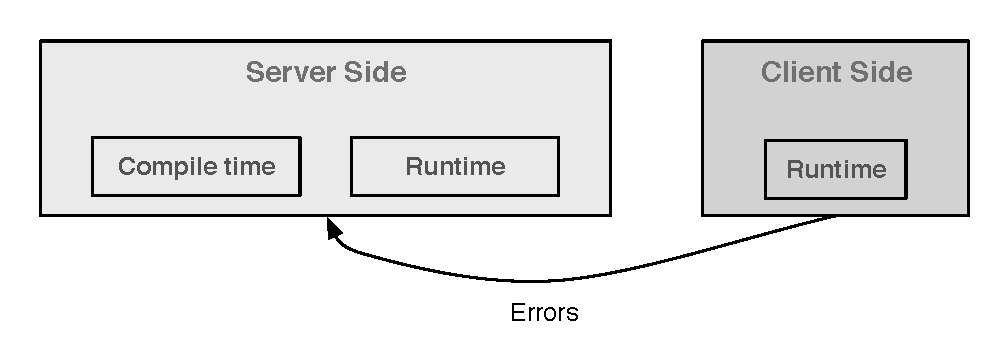
\includegraphics[width=11cm]{resources/images/MovingErrors.eps}}
		\end{center}
		\caption{Improving safe JavaScript development by trying to move errors from client side to server side.}
		\label{movingErrors}
	\end{figure}
	When considering web applications built with ASP.NET Web Forms, errors can occur both on server and client side. On server side, errors can occur on either compile time or runtime. On client side, compile time does not exist as JavaScript is an interpreted language and consequently client side errors can only occur on runtime. Client side errors will be exposed to the end users while leaving the web application in a corrupt state which is highly undesirable. Server side errors occur before the web applications is displayed on client side; if a server side error occurs, the web application is not displayed. Therefore, moving client side errors to server side can prevent a web application in a corrupt state from being exposed to the end user. 
% subsubsection subsubsection_name (end)

\subsubsection{Obtaining JavaScript-HTML Consistency} % (fold)
\label{ssub:obtaining_javascript_html_consistency}
	Compile time guarantee of the consistency between JavaScript code and HTML elements would be beneficial. Web pages typically consist of HTML elements and JavaScript source code. JavaScript is activated in response to user interactions (e.g. when clicking a button). However, due to JavaScripts interpreted nature, there is no guarantee of correct interaction between the JavaScript and the HTML elements. E.g. when calling a JavaScript function from a button click event, it is possible to have misspelled the function name which would cause a client side error. 
% subsubsection obtaining_javascript_html_consistency (end)

\subsubsection{Server-Client Portability} % (fold)
	It is beneficial to be able to generate JavaScript from compile time validated server side code. First of all, this would contribute to safe JavaScript development. Secondly, in some situations, such as form validation, it can be useful to run the same piece of code both on client and server side. As a user experience enriching feature, forms are often validated on client side, as to avoid the waiting time for a page load. However, forms have to be validated on the server side as well since the client side validation is easily bypassed (this can be done by simply disabling JavaScript in the browser). \newline
% subsubsection subsubsection_name (end)


To address these three improvements, MiCS uses Microsoft's Roslyn in combination with Script\# to generate JavaScript from C\# source code, and by extending the way ASP.NET Web Forms works with HTML elements.

\section{Reading Guide}

	This report is directed to people with interest in how JavaScript can be safely written in Microsoft ASP.NET web applications. It is assumed that the reader has a general understanding of Abstract Syntax Trees and a basic understanding of JavaScript. Third party libraries used in the project, namely Roslyn and Script\#, will be introduced and thus knowledge about these is not a prerequisite.

	This report proposes a solution where JavaScript is written safely by translating C\# to JavaScript. This approach makes it possible to execute the same code both on server and client side and is therefore called Mixed Side C Sharp (MiCS).

	This document consists of nine chapters.

	Chapter one introduces the project, the motivation behind it and its scope. Additionally it introduces the case study upon which it is based.

	Chapter two briefly introduces Microsoft ASP.NET Web Forms and the usage of Code Behind to develop web applications. Furthermore it explains why JavaScript can be considered an unsafe language.

	Chapter three introduces various technologies that can be useful to the project and describes how they can be used in combination to approach the problem definition in different ways. Furthermore an analysis is conducted in order to investigate which approach is most convenient to implement. The chosen solution is called MiCS.

	Chapter four is a short manual that describes how MiCS is used.

	Chapter five describes the MiCS project main workflow, architecture and other design decisions.

	Chapter six describes the implementation of MiCS; how types are handled and mapped, validation of mixed and client side code, mapping of ASTs and script generation.

	Chapter seven shortly describes the testing done in the MiCS project.
	
	Chapter eight evaluates the MiCS solution, reflects on the design goals set in the problem definition and discusses what future directions the project could take from here.

	Chapter nine is the report conclusion.

	In the report we use the terms developer and end user. The developer is a person that uses MiCS to write mixed side and client side code. The end user is the person that use the web application created by the developer.
	% Todo: Update reading guide as one of the last things...
	% Todo: Introduce DOM, Safety vs security, when we say JavaScript we JavaScript in the browser
	% Todo: The read should have knowledge of DSL, JavaScript (script), client server side, DOM
	% Todo: SS = ScriptSharp namespace in code examples...


\section{Problem definition}
	The problem definition has changed since the beginning of this project. Originally we wanted to represent JavaScript as an internal DSL in C\#. Instead we widened the project scope to include other possible approaches to improving JavaScript development in ASP.NET Web Forms. Below, the revised problem definition is listed.

	\begin{itemize}
		\item Study JavaScript and describe its unsafe language features.
		\item Investigate how to move JavaScript errors from client side to server side. 
		\item Investigate how to generate JavaScript from server side code in order to achieve server-client portability.
		\item Investigate how to achieve compile time guarantee of the consistency between the generated JavaScript and HTML elements.
		\item Implement and test a framework for ASP.NET Web Forms that encompassses all of the above.
	\end{itemize}

	\section{Learning goals}
		\begin{itemize}
			\item Better knowledge of JavaScript in general and its more subtle language features.
			\item Better knowledge of ASP.NET Web Forms.
		 	\item Better understanding of the difference between statically and dynamically typed languages.
			\item Better understanding of programming languages represented as abstract syntax trees.
		\end{itemize}

\section{Method}
	\begin{itemize}
	\item We will study JavaScript literature to obtain a better understanding of JavaScript and which of its features can be considered unsafe. 
	\item We will investigate which technologies can contribute to moving JavaScript errors from client side to server side, and contribute to gaining server-client portability. To address these problems, we will describe different solutions that use these technologies in combination.
	\item We will analyse and compare the solutions in order to find the one that best fits this project. 
	\item In order to achieve JavaScript-HTML consistency, we will implement the chosen solution as a framework for ASP.NET Web Forms.
	\item We will set up a unit test suite in order to ensure that the implemented framework works as expected.
	\end{itemize}

\section{Scope}
	% Todo: Do we say something about the use of DOM types is down prioritized?
	% Todo: Only JavaScript in the browser.
	As stated in the problem definition, it is the intention to generate JavaScript from server side code (C\# or F\#). However, mapping an entire language to JavaScript is unrealistic given the time constraints on this project. Therefore, the project is based on a case study concerning form validation. Only the subset of the language needed to fulfill the requirements set by the case study will be taken into account.

	\subsection{Case Study}
		A common use case of JavaScript is form validation. As mentioned earlier, form validation is a great example of a situation in which the same piece of code is necessary to run both on server and client side. Our case study concerns the validation of a registration form. Specifically, we would like to be able to:

		\begin{itemize}
			\item Validate strings using Regular Expressions to check if email addresses, postal addresses and phone numbers are correctly formatted
			\item Validate the length of strings to check that users do not enter an exceptionally long string, e.g. as their name
			\item Validate dependencies between input (conditional logic). E.g. validation of a text field depends on whether or not a check box is checked.
		\end{itemize}

		Figure~\ref{registrationForm} shows the registration form, and below, the validation criteria are explained.

		\begin{figure}
			\begin{center}
				\centerline{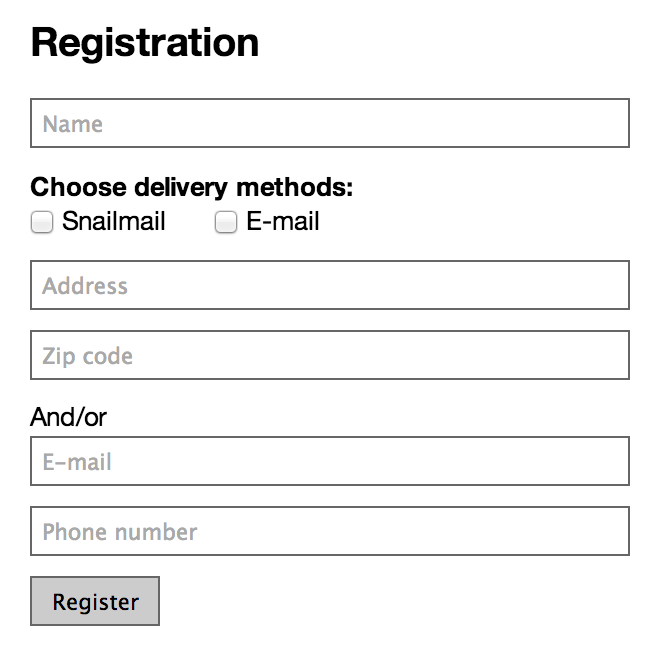
\includegraphics[width=7cm]{resources/images/registrationform.png}}
			\end{center}
			\caption{The form that we aim at validating}
			\label{registrationForm}
		\end{figure}

		\begin{itemize}
			\item The name has to consist of at least a first name and a last name, cannot be less than 5 characters long and not exceed 128 characters
			\item At least one delivery method has to be checked. If ``Snailmail'' is checked, the address and zip code fields have to be filled in. If ``E-mail'' is checked, the ``E-mail'' field has to be filled in.
			\item The address has to follow the format: \newline\newline \texttt{(streetname) (house number)[, (floor number). (TH|TV|SAL)]}\newline\newline where everything within the brackets is optional. For example, the addresses ``Amagerbrogade 125, 3.TV'' and ``Englodden 4'' are valid addresses, whereas ``Griffenfeldsgade'' and ``Svinget 34, 4'' are not.
			\item The zip code has to consist of four integer characters (Danish zip code).
			\item The e-mail address has to valid.
			\item The phone number has to consist of 8 numbers, where the first number cannot be “0” (Danish phone number).
		\end{itemize}


	% \subsection{Safety Considerations} % (fold)
	% \label{sub:safety_considerations}
	% 	This section will address some fundamental aspects of safe development that we would like to target in this project.
	% 	% There are some fundamental aspects of safe development that we will like to target in this project and which we will describe here. 

	% 	\subsubsection{Compile Time Errors vs. Runtime Errors} % (fold)
	% 	\label{ssub:compile_time_errors_vs_runtime_errors}
			
	% 		When considering web applications, errors can occur both on server side and client side. On server side, errors can occur on either compile time or runtime. On client side, compile time does not exist, and consequently errors can only occur on runtime.
	% 		Compile time errors are generally easier to debug than runtime errors and thus fixing them is often less time consuming. Client side runtime errors will be exposed to web application's end users which is highly undesirable. Because of this, one of the fundamental goals of MiCS is to move errors from client side runtime to server side (runtime or compile time, see Figure \ref{movingErrors}).

	% 		\begin{figure}
	% 			\begin{center}
	% 				\centerline{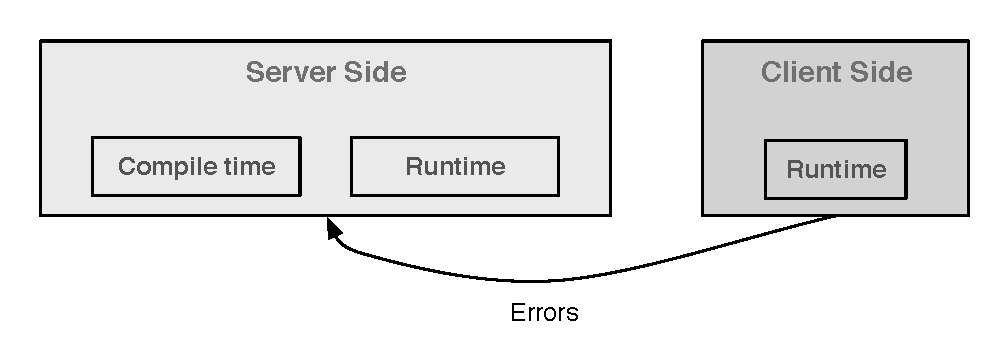
\includegraphics[width=11cm]{resources/images/MovingErrors.eps}}
	% 			\end{center}
	% 			\caption{Improving safe development by trying to move errors from client side to server side.}
	% 			\label{movingErrors}
	% 		\end{figure}
	% 	% subsubsection compile_time_errors_vs_runtime_errors (end)

	% 	\subsubsection{JavaScript-HTML Consistency} % (fold)
	% 	\label{ssub:javascript_html_consistency}
	% 		When building a web page a typical setup is a document consisting of HTML elements (DOM elements) and some client side JavaScript. The client side scripts then modifies the HTML elements in response to user interactions. There are however no guarantee of correct interaction between the JavaScript and the HTML elements. E.g. when calling a JavaScript function from a button \texttt{onclick} event it is possible to have misspelled the function name which would cause a client side error.

	% 		\begin{figure}
	% 			\begin{center}
	% 				\centerline{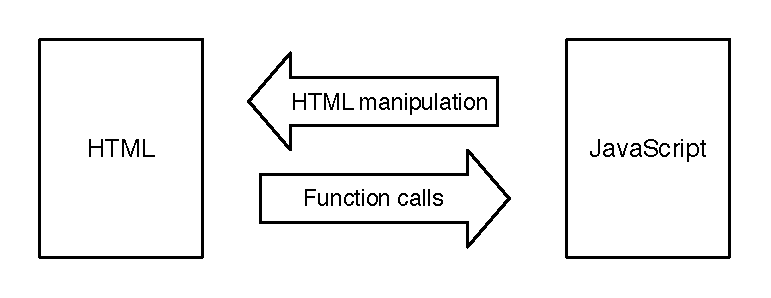
\includegraphics[width=11cm]{resources/images/javascript-html-consistency.eps}}
	% 			\end{center}
	% 			\caption{TODO: Figure text}
	% 			\label{fig:javascript_html_consistency}
	% 		\end{figure}

	% 		In the context of safe JavaScript development in the browser this can be considered a somewhat critical issue. Therefore a compile time guarantee of the consistency between JavaScript code and DOM elements (or vice versa) would be an improvement.

	% 	% subsubsection server_client_consistency (end)

	% % subsection safety_considerations (end)

	\subsection{Focus} % (fold)
	\label{sub:focus}
		This project primarily serves as a proof-of-concept and therefore the main focus will be to generate JavaScript that actually works, and can fulfill the requirements set by the case study. 

		This project will only consider solutions that can be used with Microsoft's ASP.NET Web Forms.

		The quality of the generated JavaScript will not be assessed. The primary reason for this is that the suggested solution will be using parts of the Script\# framework to generate the actual JavaScript source code.

		Likewise overall performance will not be analyzed due to the time constraints on the project.
	% subsection focus (end)


\section{Target Audience} % (fold)
\label{sec:section_name}
	The target audience is developers who create web applications using ASP.NET Web Forms with C\# where correctness is of high priority. This implies that the developer aims at displaying a 100\% working web application or nothing at all. An error message is preferred over an application in a corrupt, or partly corrupt, state.
% section section_name (end)


% chapter introduction (end)




